\documentclass[10pt,twocolumn,letterpaper]{article}
\usepackage{comment}

\usepackage[utf8]{inputenc}
\usepackage{caption}
\usepackage{tabularx}
\captionsetup[table]{skip=20pt}
\usepackage{cvpr}
\usepackage{mathptmx}
\usepackage{graphicx}
\usepackage{amsmath}
\usepackage{siunitx}
\usepackage{amssymb}
\usepackage{tikz}
\usepackage{pgfplots}
\usepackage{subcaption}
\usepackage{bm,color}
\usetikzlibrary{arrows.meta}
\usetikzlibrary{shapes, arrows}
\usepackage{graphics}
\usepackage{pifont}
\pgfplotsset{compat=newest}
\usepackage{blindtext}

\usepackage[pagebackref=true,breaklinks=true,letterpaper=true,colorlinks,bookmarks=false]{hyperref}


\newcommand{\cmark}{\ding{51}}
\newcommand{\xmark}{\ding{55}}

% Init and set plot shapes
\newlength\figH
\newlength\figW
\setlength{\figH}{4cm}
\setlength{\figW}{8cm}

% Input tud colors
\input{TUDColors.tex}

% Math styles
\newcommand{\Vector}[1]{\boldsymbol{#1}}
\newcommand{\Matrix}[1]{\boldsymbol{\MakeUppercase{#1}}}
\newcommand{\Tensor}[1]{\boldsymbol{\mathrm{\MakeUppercase{#1}}}}
\newcommand{\Set}[1]{\mathbb{#1}}
\newcommand{\Mean}[1]{\mathbb{E}\left(#1\right)}
\newcommand{\Var}[1]{\mathrm{Var}\left(#1\right)}
\newcommand{\Cov}[1]{\mathrm{Cov}\left(#1\right)}
\newcommand{\Gaussian}[1]{\mathcal{N}\left(#1\right)}

\cvprfinalcopy

\def\httilde{\mbox{\tt\raisebox{-.5ex}{\symbol{126}}}}

\setcounter{page}{1}
\begin{document}

\title{DeepFovea++: Reconstruction and Super-Resolution for Natural Foveated Rendered Videos}

\author{
    Christoph Reich\\
    TU Darmstadt\\
    {\tt\small christoph.reich@stud.tu-darmstadt.de}
    
    \and
    Marius Memmel\\
    TU Darmstadt\\
    {\tt\small marius.memmel@stud.tu-darmstadt.de}
    
    \and
    Jonas Henry Grebe\\
    TU Darmstadt\\
    {\tt\small jonas.grebe@stud.tu-darmstadt.de}
}


\twocolumn[{%
\renewcommand\twocolumn[1][]{#1}%
\maketitle
\begin{center}
    \centering
    \includegraphics[width=\textwidth]{figures/input.png}\\\vspace{-0.1cm}
    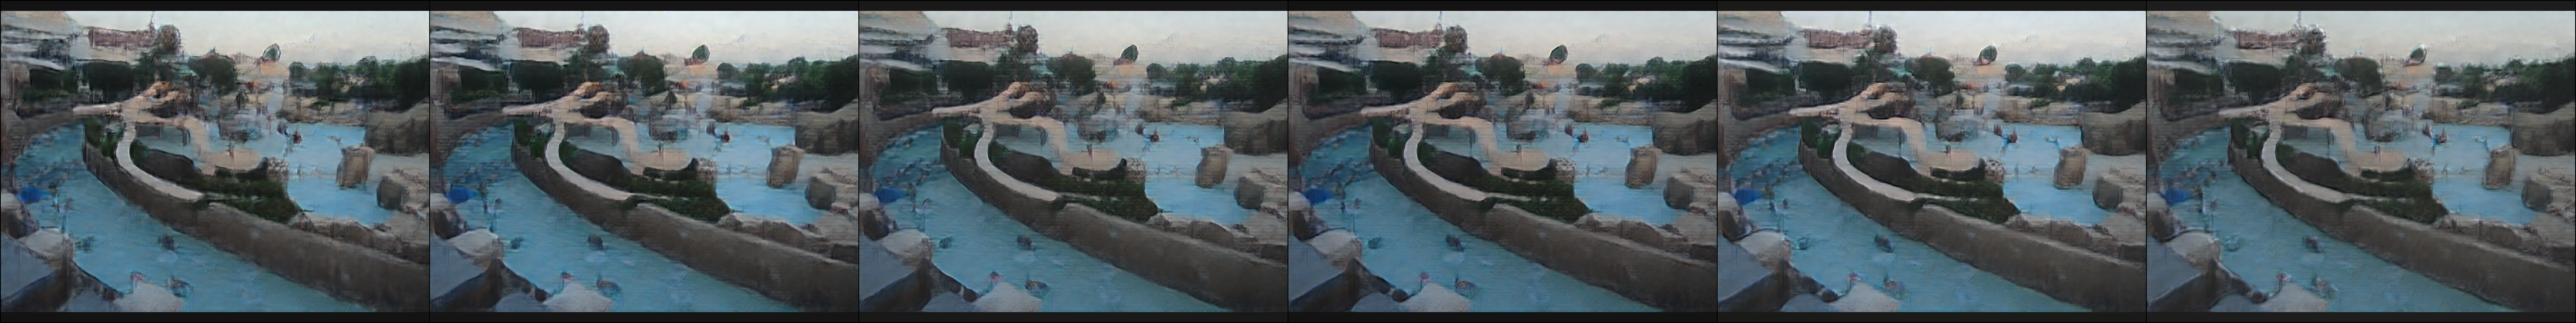
\includegraphics[width=\textwidth]{figures/prediction.png}\\\vspace{-0.1cm}
    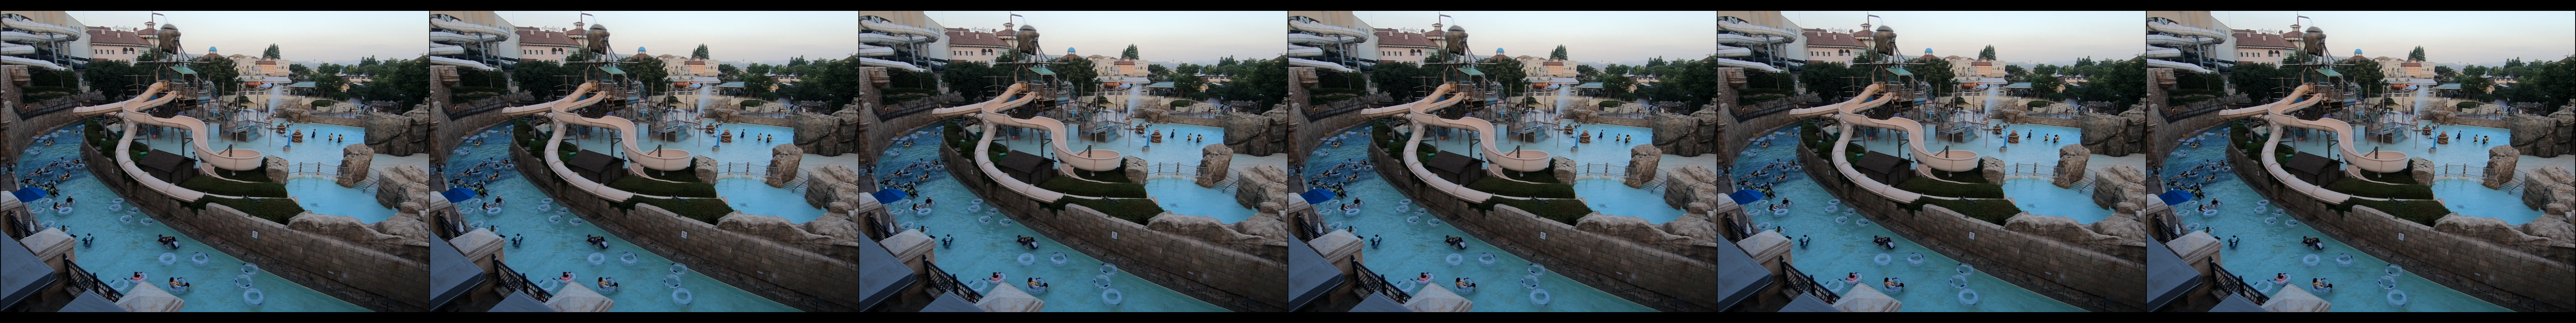
\includegraphics[width=\textwidth]{figures/label.png}\\
    \captionof{figure}{First results of our proposed DeepFovea++ technique. The fovea sampled input sequences of low resolution (192 X 256) image frames can be seen on the top. The reconstructed super-resolution (768 X 1024) prediction sequence is shown in the middle, and the corresponding label at the bottom.}
    \label{fig:results}
\end{center}%
}]

\begin{abstract}
Image super-resolution is a well-known problem in the computer vision community. Recent papers extended the problem of super-resolution to videos and showed amazing results. On the other hand deep learning based fovea sampled image reconstruction has drawn some popularity since the DeepFovea publication of Facebook AI. DeepFovea showed outstanding results, however, the proposed reconstruction network was only able to reconstruct relatively low-resolution images of $128\times128$ pixels. We want to revisit the DeepFovea architecture to perform fovea sampled video reconstruction and super-resolution at once. A first version of out idea is already available at \url{https://github.com/ChristophReich1996/DeepFoveaPP_for_Video_Reconstruction_and_Super_Resolution}.
\end{abstract}

\section{What we want to do?}
We want to combine the problems of super-resolution \cite{valillasuperres} and fovea sampled video reconstruction \cite{kaplanyan2019deepfovea}, to build a more general convolutional neural network (CNN) \cite{cnn} based algorithm. Since to our knowledge, there is currently no algorithm available that can perform these two tasks at once, so we could push the development of CNN algorithms a bit further with our work.

\section{Why project is this important?}
This work could lead, as mentioned earlier, to a more general CNN based algorithm. Furthermore, we possibly could hit the boundary of the capability of CNNs. Which would be also interesting to discover. Besides the theoretical aspects, real-world use-cases like virtual reality could benefit from our work. \cite{kaplanyan2019deepfovea}

\section{Why project is it interesting for you?}
All of us are interested in deep learning for computer vision. In the last semester, we (Marius \& Christoph) already completed the project-lab deep learning in computer vision. So we already have a strong prior knowledge, regarding deep learning in computer vision.
Jonas, on the other hand, has also experience in the field of deep learning in computer vision by building own projects, \href{https://github.com/jonasgrebe/tf-pokemon-generation}{see}. 

\section{How we plan to approach the solution?}
We want to build our project on top of the DeepFovea architecture, published by Facebook AI \cite{kaplanyan2019deepfovea}. To achieve video super-resolution we plan to use a deformable convolution approach similar to \cite{deformablesuperres, deformableconv}. We are also interested to apply the adaptive robust loss function by Jonathan Barron \cite{adaptiveroubustloss}. To train, validate and test our architecture we used, in our first experimental tests, the REDS dataset, which included natural video sequences. \cite{REDS}

\section{What we already achieved}
Due to the corona-virus free time, we already managed to build an experimental PyTorch \cite{pytorch} version of our idea. The first tests showed good results as can be seen in figure \ref{fig:results}. We plan the optimize our approach future and to achieve better results and a clean codebase.

{
    \bibliographystyle{ieee}
    \bibliography{egbib}
}

\end{document}